\documentclass[a4paper]{article}
\usepackage[14pt]{extsizes} % для того чтобы задать нестандартный 14-ый размер шрифта
\usepackage[left=1.5cm,right=1.5cm,top=2cm,bottom=2cm]{geometry}
\usepackage{multirow}
\usepackage{parallel}
\usepackage {graphicx}
\usepackage{multicol}
\usepackage[utf8x]{inputenc} % указать кодировку русского текста
\usepackage[russian]{babel} % указать, что язык текста - русский
\usepackage{fancyhdr}
\pagestyle{fancy}
\usepackage{graphicx}
\graphicspath{{pictures/}}
\DeclareGraphicsExtensions{.pdf,.png,.jpg, .jpeg}
\usepackage{tocloft}
\usepackage{wrapfig}
\usepackage{tikz}

\usepackage{enumitem}
\setlist[enumerate,itemize]{leftmargin=0pt,itemindent=2.7em}
\renewcommand{\cftsecleader}{\cftdotfill{\cftdotsep}}
\begin{document} 
\large
\noindent \textbf{Лабораторная работа 4.7.1: Двойное лучепреломление}\\
\\
\normalsize
\textbf{М.Шлапак}\\
\line(1,0){18cm}\\
\\
\footnotesize
\textit{Изучена зависимость показателя преломления необыкновенной волны от направления в двоякопреломляющем кристалле; определены главные показатели преломления обыкновенной и необыкновенной волны в кристалле; проведено наблюдение эффекта полного внутреннего отражения.}\\
\\
\textit{\textbf{Ключевые слова:} показатель преломления, необыкновенная волна, обыкновенная волна, двойное лучепреломление, призма, преломляющий угол, исландский шпат}\\
\fancyhead[L] {Двойное лучепреломление, М.Шлапак}

\begin{multicols}{2}

\begin{enumerate}
\small
\item \textbf{Введение}\\ 
\noindent Одним из важных видов кристаллов являются оптически одноосные кристаллы. Помимо своих простейших оптических свойств, они также имеют наибольшее практическое значение. Итак, оптически одноосные кристаллы - это кристаллы, свойства которых обладают симметрией вращения относительно некоторого направления, называемого оптической осью кристалла. Это значит, что тензор инерции диэлектрической проницаемости имеет несколько более упрощенный вид, состоящий всего из двух компонент: продольной и поперечной. Оказывается, что свет преломляется на грани призмы, сделанной из оптически одноосного кристалла, в двух направлениях, создавая две перпендикулярно поляризованные относительно друг друга волны: обыкновенную и необыкновенную, скорость которых, вообще говоря, не совпадает - у обыкновенной она является константой, а у необыкновенной зависит от направления распространения. В связи с чем, показатели преломления для двух волн тоже делаются отличными. В данной работе как раз-таки изучалось явление двойного лучепреломления в призме исландского шпата, поскольку в ней достигается наиболее значимое различие показателей преломления обыкновенной и необыкновенной волны. Немалый вклад в успешное выполнение работы также внёс поляризатор, с помощью которого удалось отделить обыкновенную и необыкновенную волны.\\
\item \textbf{Теоретические основы}
\begin{enumerate}

\item \textbf{Плоские волны в кристаллах}
\begin{equation} \label{trivial}
\hbox{rot} \vec{H} = \frac{1}{c}\frac{\partial \vec{D}}{\partial t}, \hbox{rot} \vec{E} = -\frac{1}{c}\frac{\partial \vec{B}}{\partial t} 
\end{equation}
Если среды прозрачны и однородны то в них распорстраняются волны:
\begin{equation}
\vec E = \vec{E}_0 e^{i(\omega t - \vec{k}\vec{r})}, \vec{H} = \vec{H}_0e^{i(\omega t - \vec{k}\vec{r})}
\end{equation}
Введем единичный вектор нормали к скорости распространения волны $\vec{N}$ и направим его вдоль скорости, тогда
\begin{equation}
\vec{D} = -\frac{c}{v}\left[\vec{N}, \vec{H}\right], \vec{B} = \frac{c}{v}\left[  \vec{N}, \vec{E}\right]
\end{equation}
\item \textbf{Оптические одноосные кристаллы}
Введем \textit{тензор диэлектрической проницаемости} $\varepsilon$ ($\vec{D} = \varepsilon \vec{E}$). Все его значения описываются эллипсоидом инерции. 

В кристаллах этот эллипсоид --- эллипсоид вращения. В них оптическая ось --- ось вращения эллипсоида. В них принято обозначать $\varepsilon_{\parallel} = \varepsilon_z, \varepsilon_{\perp} = \varepsilon_x = \varepsilon_y$

\begin{equation}
\vec{D}_{\parallel} = \varepsilon_{\parallel} \vec{E}_{\parallel},\vec{D}_{\perp} = \varepsilon_{\perp} \vec{E}_{\perp} 
\end{equation}

Можно показать, что угол $\theta$ между волновой нормалью и осью вращения эллипсоида при разделении $\vec{D}$ на $\vec{D}_e$ --- лежащая в главном сечении и $\vec{D}_o$ --- нормальная составляющая такой, что
\begin{equation}
\sin \theta = \frac{D_{e\parallel}}{D_e}, \cos \theta = \frac{D_{e\perp}}{D_e}
\end{equation}
\begin{equation}
n = \frac{1}{\sin A}\sqrt{\sin^2 \varphi_1 + \sin^2 \varphi_2 + 2 \sin \varphi_1 \sin \varphi_2 \cos A}
\end{equation}
\begin{equation}
\cos \theta = \frac{\sin \varphi_1}{n}
\end{equation}
Из этого, если $n_o - n_e \ll n_o$ и $n_e$, то 
\begin{equation}
n(\theta) \approx n_e + (n_o - n_e) \cos^2 \theta
\end{equation}
%\newpage
\item \textbf{Двойное лучепреломление в призме исландского шпата}\\
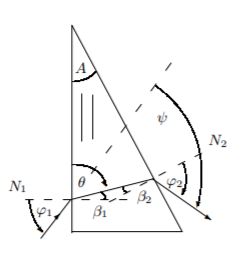
\includegraphics[width = 4.5cm]{1}\\
Можно посчитать показатель преломления изотропной среды по формуле 
\begin{equation}
n = \frac{\sin\left(\frac{\psi_m + A}{2}\right)}{\sin \left(\frac{A}{2}\right)}
\end{equation}
Здесь $\psi_m$  --- минимальный угол, на который призма преломляет луч.
Если призма неизотропна, то этой формулой, строго говоря, можно воспользоваться только для обыкновенной волны, которая, как это было показано ранее, распространяется так же, как и в изотропной среде.
\end{enumerate} 
\item \textbf{Экспериментальная установка}
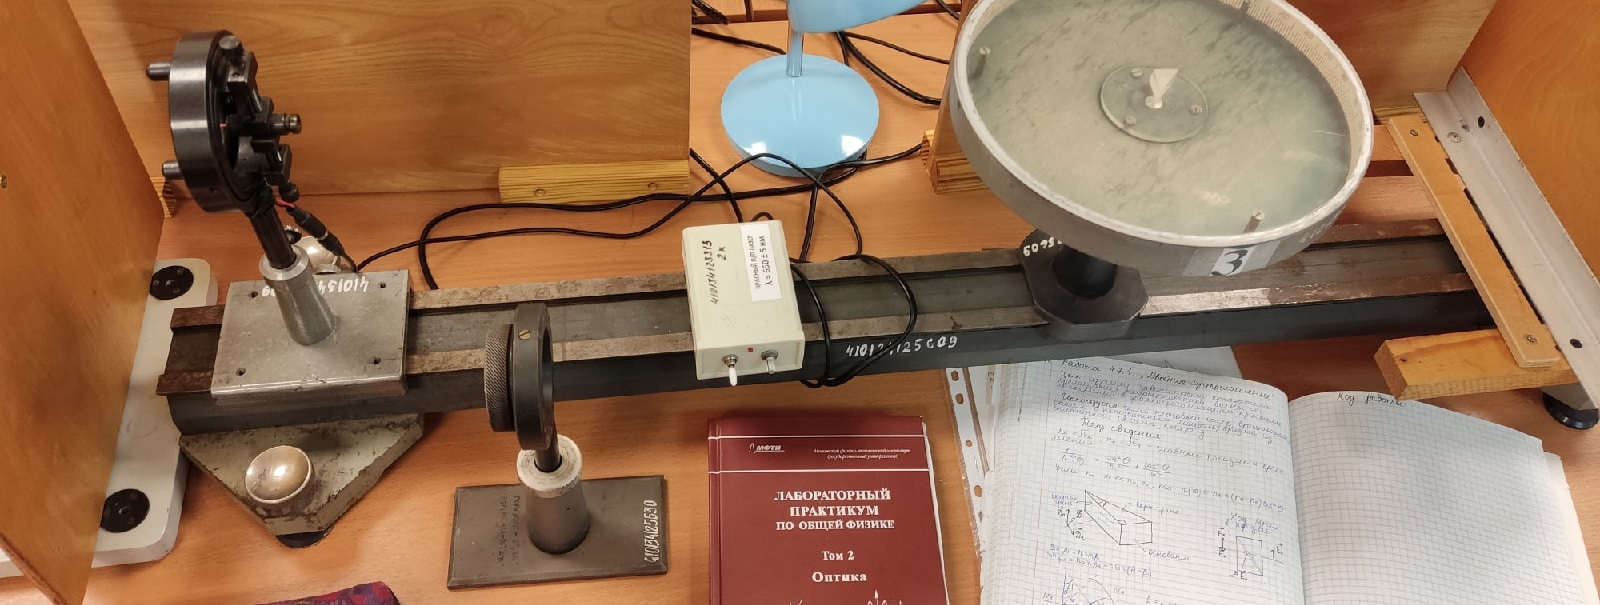
\includegraphics[width=9.0cm]{exp1}\\
\\
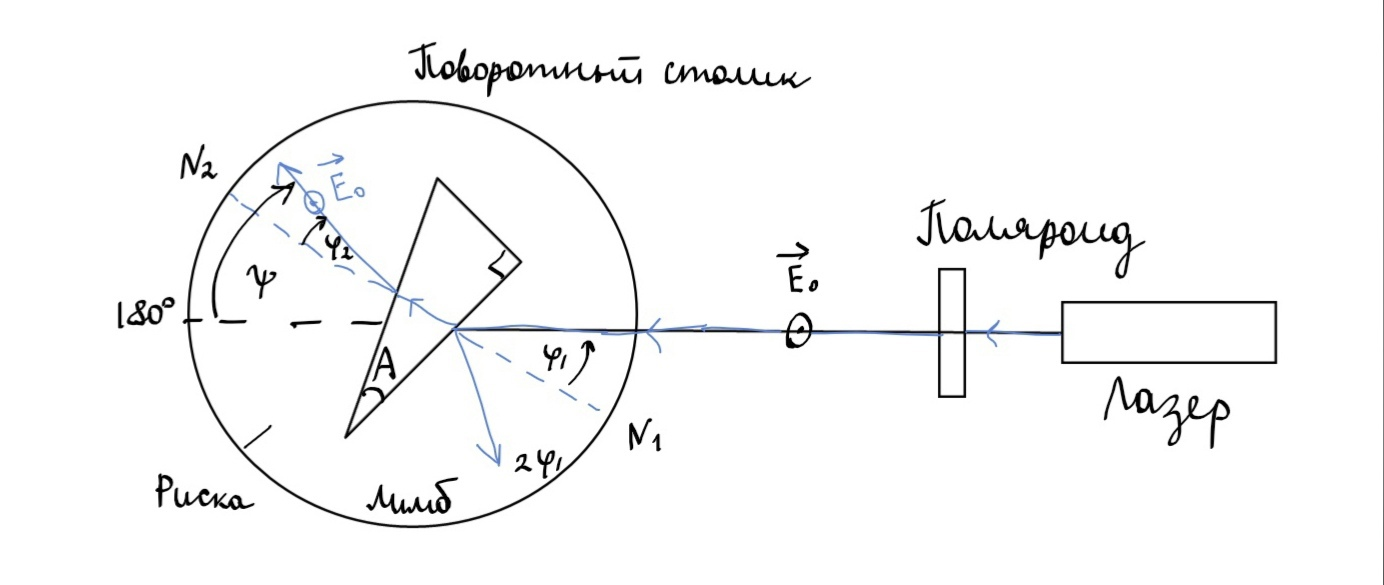
\includegraphics[width=9.5cm]{exp2}\\
\item \textbf{Результаты эксперимента}\\
В данной работе преломляющий угол призмы А, главные показатели преломления обыкновенной и необыкновенной волн определяются 3 способами. Точность расчётов в большей степени зависит от юстировки системы.\\
\begin{enumerate}
\item \textbf{Юстировка}\\
1) Определим угол А при вершине призмы. Для этого запишем положение отсчётной риски на лимбе сначала для длинного катета, а потом для гипотенузы в том случае, когда луч, отраженный от входящей грани (катет или гипотенуза), идёт точно назад.\\
А = $ 180 - (\phi_1 - \phi_0)$\\
$$\phi_0 = 194,0^{\circ} \pm 0,5^{\circ} \; \; \hbox{- катет}$$
$$\phi_1 = 336,0^{\circ} \pm 0,5^{\circ} \; \; \hbox{- гипотенуза}$$
Таким образом, преломляющий угол призмы: $$A = 38,0^{\circ} \pm 1,0^{\circ}$$
\item \textbf{Поиск показателей преломления}
2)Далее определяем разрешающую способность поляризатора, чтобы впоследствии уметь отделять обыкновенный луч от необыкновенного. \\
3) Получим на поворотном столике изображения лучей обыкновенной волны и необыкновенной волны:\\
При разрешенном направлении поляризатора в $320^{\circ}$ запирается горизонтальная поляризация (запираем необыкновенный луч)\\
При разрешенном направлении в $230^{\circ}$ запирается вертикальная поляризация (слабый обыкновенный луч).\\
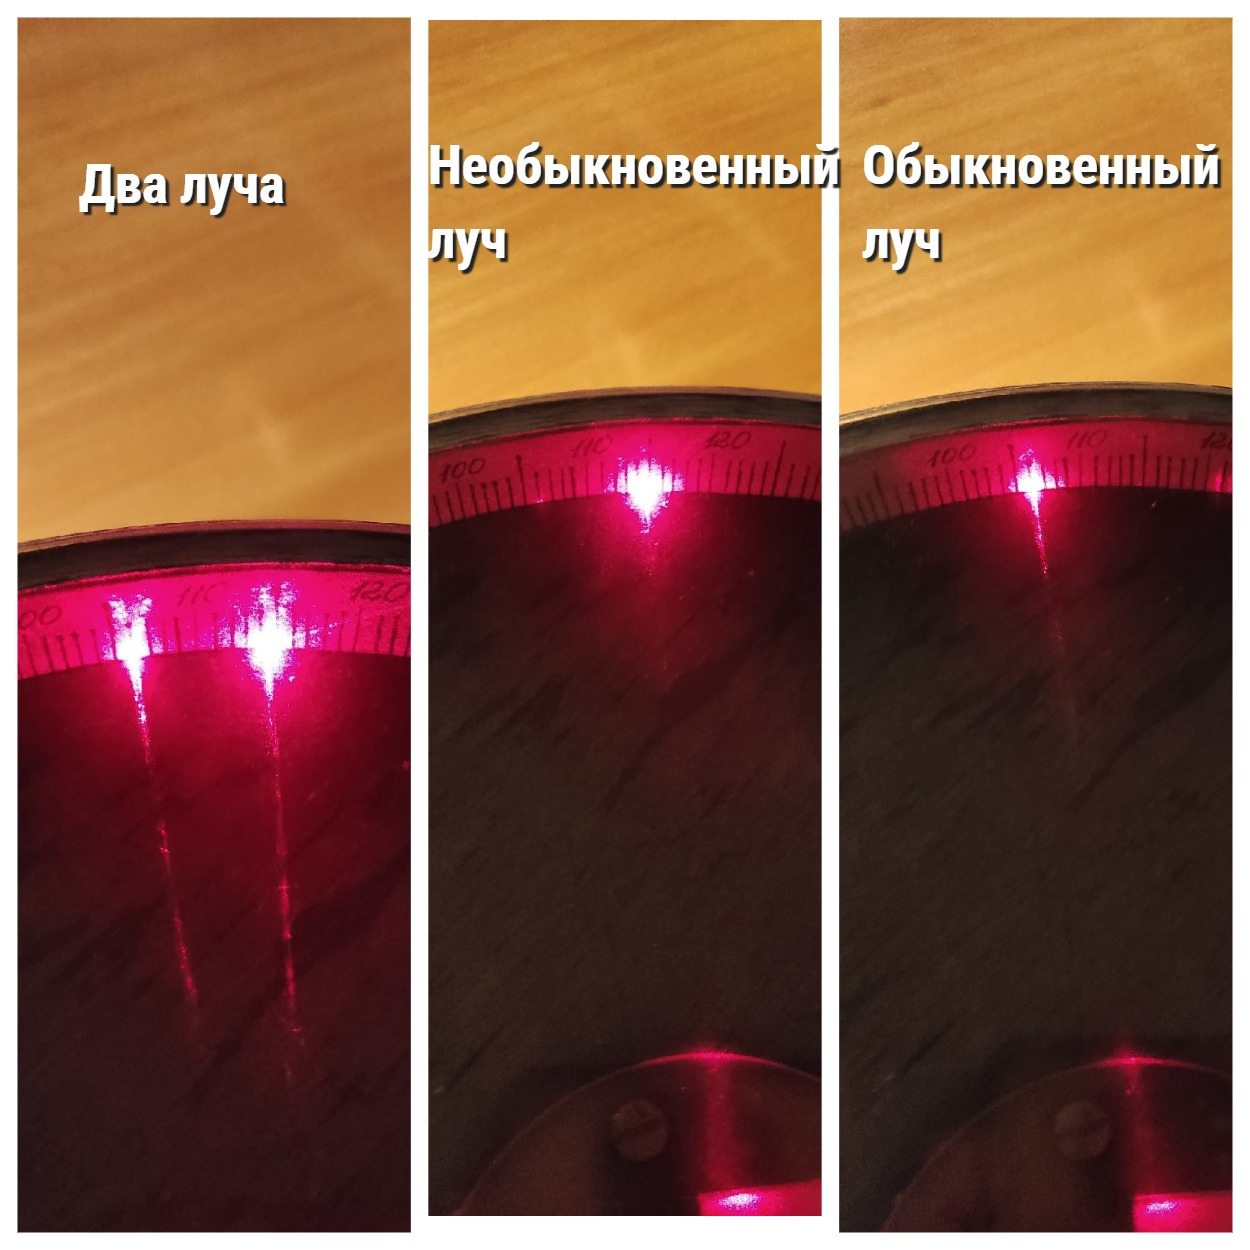
\includegraphics[width=9.5cm]{exp6}\\
4) Вращая столик с призмой, снимем зависимость углов отклонения на выходе из призмы для обыкновенной и необыкновенной волн от угла падения на призму, взяв диапазон $10-70^{\circ}$ через $5^{\circ}$.\\
5) С помощью формул (6) и (7) найдем $n_0$ и $n_e(\theta)$. Построим по рассчитаным значениям графики и убедимся, что показатель преломления обыкновенной волны не зависит от направления распространения, а необыкновенной - зависит.\\ Определим главные направления $n_0$ и $n_e$:\\
$$n_0 = 1,64 \pm 0,02$$
$$n_e = n_e(0) = 1,47 \pm 0,02$$ 
\end{enumerate}
\noindent 6) Из основной серии измерений определим средние значения углов наименьшего отклонения $\phi_m$:
$$\phi_{mo} = 26,0 \pm 1,0$$
$$\phi_{me} = 20,0 \pm 1,0$$
Рассчитаем главные показатели преломления по формуле (9):
$$n_o = 1,63 \pm 0,10$$
$$n_e = 1,49 \pm 0,08$$
7) Определим углы полного внутреннего отражения:
$$2\phi_{1o} = (4,0 \pm 0,5)^{\circ}$$
$$2\phi_{1e} = -(12,0 \pm 0,5)^{\circ}$$
Рассчитаем значения $n_o$ и $n_e$ по формуле (6), не забывая, что угол $\phi_2 = 90^{\circ}$:
$$n_o = 1,67 \pm 0,02$$
$$n_e = 1,49 \pm 0,02$$
\item \textbf{Заключение}\\
В данной работе было исследовано двойное лучепреломление в призме исладнского шпата, а также были определены главные показатели преломления $n_e$ и $n_o$ тремя способами:\\
1) По зависимости входного и выходного углов для обыкновенной и необыкновенной волн\\
2) По углам наименьшего отклонения для обыкновенной и необыкновенной волн\\
3) С поомщью полного внутреннего отражения\\
 Полученные результаты хорошо соотносятся с табличными значениями $n_o = 1,655$ и $n_e = 1,485$\\
 \\
\textit{1. Общий курс физики. Оптика, Д.В.Сивухин}\\
\textit{2. Лабораторный практикум по общей физике. Оптика, А.В. Максимычев}\\
 \end{enumerate}
\end{multicols}
 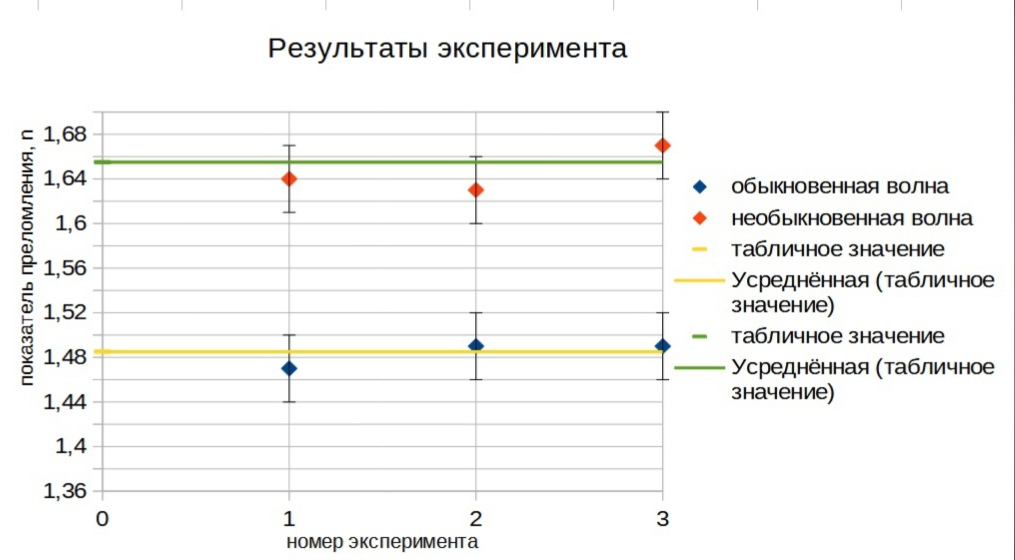
\includegraphics[width = 18cm]{g3}\\
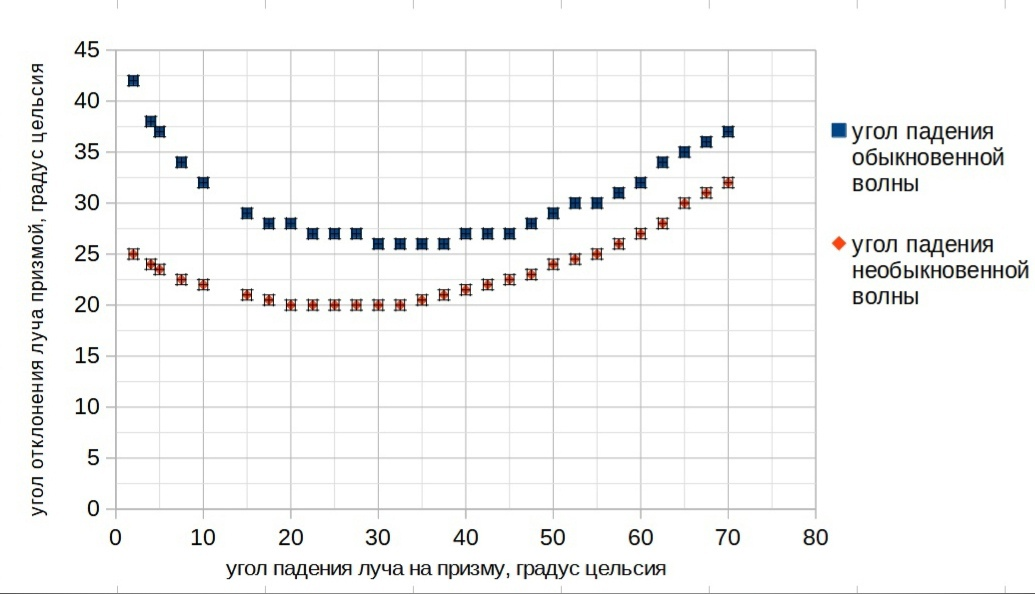
\includegraphics[width=18cm]{g11}\\
\\
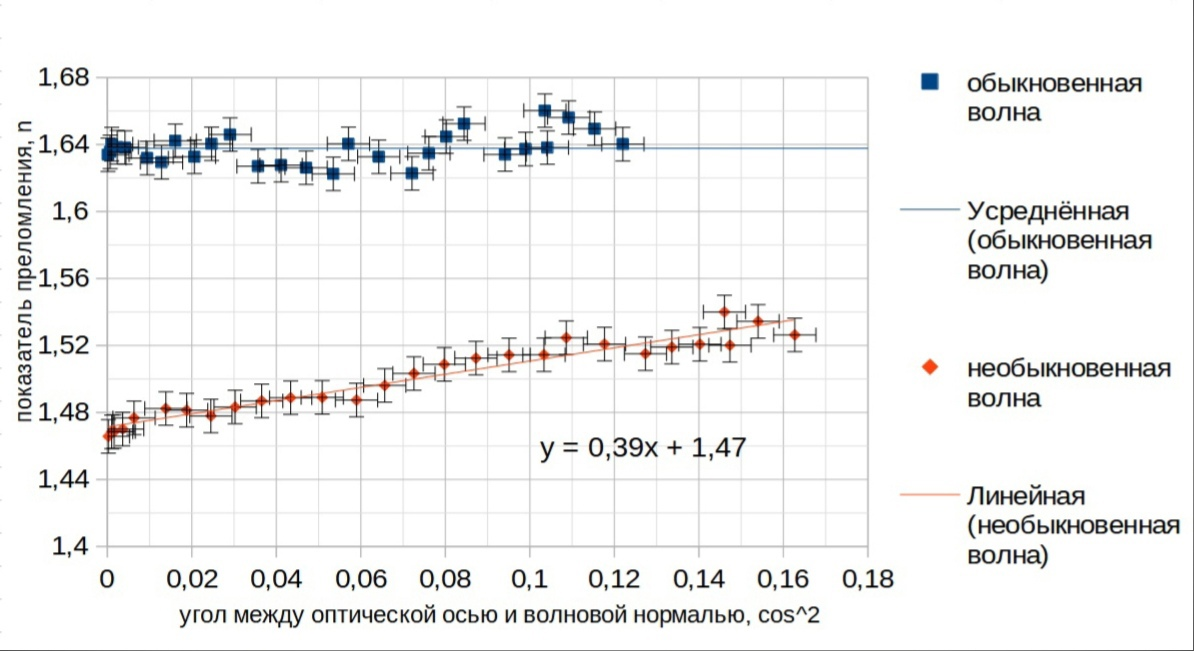
\includegraphics[width=18cm]{g22}\\
\end{document}